\documentclass[11pt,compress,t,notes=noshow, xcolor=table]{beamer}
\usepackage[]{graphicx}\usepackage[]{color}
% maxwidth is the original width if it is less than linewidth
% otherwise use linewidth (to make sure the graphics do not exceed the margin)
\makeatletter
\def\maxwidth{ %
  \ifdim\Gin@nat@width>\linewidth
    \linewidth
  \else
    \Gin@nat@width
  \fi
}
\makeatother

\definecolor{fgcolor}{rgb}{0.345, 0.345, 0.345}
\newcommand{\hlnum}[1]{\textcolor[rgb]{0.686,0.059,0.569}{#1}}%
\newcommand{\hlstr}[1]{\textcolor[rgb]{0.192,0.494,0.8}{#1}}%
\newcommand{\hlcom}[1]{\textcolor[rgb]{0.678,0.584,0.686}{\textit{#1}}}%
\newcommand{\hlopt}[1]{\textcolor[rgb]{0,0,0}{#1}}%
\newcommand{\hlstd}[1]{\textcolor[rgb]{0.345,0.345,0.345}{#1}}%
\newcommand{\hlkwa}[1]{\textcolor[rgb]{0.161,0.373,0.58}{\textbf{#1}}}%
\newcommand{\hlkwb}[1]{\textcolor[rgb]{0.69,0.353,0.396}{#1}}%
\newcommand{\hlkwc}[1]{\textcolor[rgb]{0.333,0.667,0.333}{#1}}%
\newcommand{\hlkwd}[1]{\textcolor[rgb]{0.737,0.353,0.396}{\textbf{#1}}}%
\let\hlipl\hlkwb

\usepackage{framed}
\makeatletter
\newenvironment{kframe}{%
 \def\at@end@of@kframe{}%
 \ifinner\ifhmode%
  \def\at@end@of@kframe{\end{minipage}}%
  \begin{minipage}{\columnwidth}%
 \fi\fi%
 \def\FrameCommand##1{\hskip\@totalleftmargin \hskip-\fboxsep
 \colorbox{shadecolor}{##1}\hskip-\fboxsep
     % There is no \\@totalrightmargin, so:
     \hskip-\linewidth \hskip-\@totalleftmargin \hskip\columnwidth}%
 \MakeFramed {\advance\hsize-\width
   \@totalleftmargin\z@ \linewidth\hsize
   \@setminipage}}%
 {\par\unskip\endMakeFramed%
 \at@end@of@kframe}
\makeatother

\definecolor{shadecolor}{rgb}{.97, .97, .97}
\definecolor{messagecolor}{rgb}{0, 0, 0}
\definecolor{warningcolor}{rgb}{1, 0, 1}
\definecolor{errorcolor}{rgb}{1, 0, 0}
\newenvironment{knitrout}{}{} % an empty environment to be redefined in TeX

\usepackage{alltt}
\newcommand{\SweaveOpts}[1]{}  % do not interfere with LaTeX
\newcommand{\SweaveInput}[1]{} % because they are not real TeX commands
\newcommand{\Sexpr}[1]{}       % will only be parsed by R



\usepackage[english]{babel}
\usepackage[utf8]{inputenc}

\usepackage{dsfont}
\usepackage{verbatim}
\usepackage{amsmath}
\usepackage{amsfonts}
\usepackage{bm}
\usepackage{csquotes}
\usepackage{multirow}
\usepackage{longtable}
\usepackage{booktabs}
\usepackage{enumerate}
\usepackage[absolute,overlay]{textpos}
\usepackage{psfrag}
\usepackage{algorithm}
\usepackage{algpseudocode}
\usepackage{eqnarray}
\usepackage{arydshln}
\usepackage{tabularx}
\usepackage{placeins}
\usepackage{tikz}
\usepackage{setspace}
\usepackage{colortbl}
\usepackage{mathtools}
\usepackage{wrapfig}
\usepackage{bm}
\usetikzlibrary{shapes,arrows,automata,positioning,calc,chains,trees, shadows}
\tikzset{
  %Define standard arrow tip
  >=stealth',
  %Define style for boxes
  punkt/.style={
    rectangle,
    rounded corners,
    draw=black, very thick,
    text width=6.5em,
    minimum height=2em,
    text centered},
  % Define arrow style
  pil/.style={
    ->,
    thick,
    shorten <=2pt,
    shorten >=2pt,}
}
\usepackage{subfig}


% Defines macros and environments
\input{../../style/common.tex}
% \input{common.tex}

%\usetheme{lmu-lecture}
\newcommand{\titlefigure}{figure/benchmark_curve_iter_all_median.png}
\newcommand{\learninggoals}{
\item Understand the idea of grid search
\item Understand the idea of random search
\item Be able to discuss advantages and disadvantages of the two methods}
\usepackage{../../style/lmu-lecture}

\let\code=\texttt
\let\proglang=\textsf

\setkeys{Gin}{width=0.9\textwidth}

\title{Introduction to Machine Learning}
% \author{Bernd Bischl, Christoph Molnar, Daniel Schalk, Fabian Scheipl}
\institute{\href{https://compstat-lmu.github.io/lecture_i2ml/}{compstat-lmu.github.io/lecture\_i2ml}}
\date{}

\setbeamertemplate{frametitle}{\expandafter\uppercase\expandafter\insertframetitle}



\begin{document}

% Load all R packages and set up knitr

% This file loads R packages, configures knitr options and sets preamble.Rnw as parent file
% IF YOU MODIFY THIS, PLZ ALSO MODIFY setup.Rmd ACCORDINGLY...
% Defines macros and environments
\input{../../latex-math/basic-math.tex}
\input{../../latex-math/basic-ml.tex}
\input{../../latex-math/ml-lm.tex}
\input{../../latex-math/ml-automl.tex}



\lecturechapter{Hyperparameter Tuning - Example and Practical Hints}
\lecture{Introduction to Machine Learning}
\sloppy

\begin{frame}[allowframebreaks]{Scaling and Ranges}

\begin{itemize}
	\item Knowledge about hyperparameters can help to guide the optimization
	\item E.g., it can be beneficial to optimize hyperparameters on a non-uniform scale.
\end{itemize}

    % \vspace{0.2cm}
Example: regularization hyperparameter on log-scale

\begin{itemize}
    \item Many ML algorithms have non-neg. hyperparameters (e.g. regularization constant), for which it can make sense to try out very small and very large values during tuning 
    % \item Standard examples are regularization parameters       
    \item Usual trick: put on log-scale: $C$ of SVM: $[2^{-15}, 2^{15}] = [0.00003, 32768]$
	% \item The distance between $10$ and $20$ should be the same as between $0.1$ and $0.2$.
  % \item We might want to sample here from from a log-scale, e.g., $[2^{\conf_l}, 2^{\conf_u}]$ with $\conf_l = -5$ and $\conf_u = 5$.
\end{itemize}

\begin{figure}[htb]
\centering
% from AutoML lecture: 
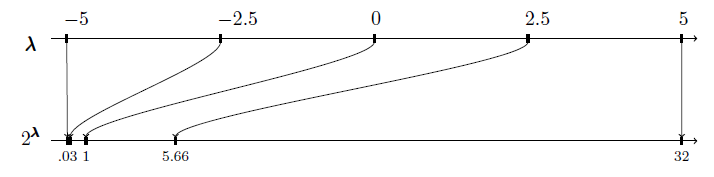
\includegraphics[width=0.9\textwidth]{figure_man/scaling-ranges-tikz.PNG}
  % \begin{tikzpicture}[auto]
  %   \draw [->](-0.3,0)-- (12.3,0) coordinate;
  %   \draw [->](-0.3,-2)-- (12.3,-2) coordinate;
  %   % \foreach \x/\xtext/\xxtext in {-15/-15/0.000031, -10/-10/ , -5/-5/, 0/0/1, 5/5/32, 10/10/1024, 15/15/32768} {
  %   
  %   \def\xM{5} % max exponent
  %   \def\xW{12} % max width in cm
  %   
  %   \foreach \xv/\xtext/\xxtext in {-5/-5/.03, -2.5/-2.5/, 0/0/1, 2.5/2.5/5.66, 5/5/32} {
  %     \def\xA{{(\xv + \xM) * (\xW / (2 * \xM))}} %untrafoed val in cm (0 to 12)
  %     \def\xB{{\xW * 2^(\x-\xM)}} %trafoed val in cm
  %     \draw [very thick] (\xA,-2pt) -- ++(0, 4pt) node[xshift = -6pt, yshift=-3pt,anchor=south west,baseline]{\strut$\xtext$};
  %     \draw [very thick] (\xB,-2cm+2pt) -- ++(0,-4pt) node[anchor=north]{\scriptsize $\xxtext$};
  %     \draw [->] (\xA,-2pt) .. controls (\xA,-0.5) and (\xB,-1.5) .. (\xB,-2cm+2pt);
  %   }
  %   \node[] at (-0.7,-0.1) (t1) {$\bm{\lambda}$};
  %   \node[] at (-0.7,-1.9) (t2) {$2^{\bm{\lambda}}$};
  % \end{tikzpicture}

\end{figure}

\framebreak

    \begin{itemize}
        \item Similar to the scale, e.g., linear or logarithmic, upper and lower bounds for hyperparameters have to be specified as many optimizers require them
        \item Setting these correctly usually requires deeper knowledge about the inner workings of the ML method and a lot of practical experience
        \item Furthermore, if $\bm{\hat{\lambda}}$ is close to the border of $\bm{\Lambda}$ the ranges should be increased (or a different scale should be selected), but many algorithms do not do this automatically
        \item Meta-Learning can help to decide which hyperparameters should be tuned in which ranges
    \end{itemize}
    % \vspace{0.5cm}
    % Example:
    % \begin{itemize}
    %         \item The ranges for $\text{cost} \in [10^{-3}, 10^3]$ and $\gamma \in [10^{-3}, 10^3]$ are rather small.
    %         \item More common would be ranges like $\text{cost} \in [2^{-15}, 2^{15}]$ and $\gamma \in [2^{-15}, 2^{15}]$.
    % \end{itemize}

\end{frame}

\begin{frame}{Default Heuristics}

    \begin{itemize}
            \item Instead of using static defaults, we sometimes can compute hyperparamter defaults heuristically, based on simple data characteristics.
            \item A lot faster than tuning and sometimes can work well,
                although not many guarantees exists and it is often unclear how well this works across many different data scenarios
            \item Well-known example: Number of random features to consider for splitting in random forest: $\text{mtry} = \sqrt{p}$, where $p$ is total number of features.
            \item For the RBF-SVM a data dependent default for the $\gamma$ parameter (inverse kernel width) can be computed by using the (inverse of the) median of the pairwise distances $\|\xv-\xtil\|$between data points (or a smaller random subset for efficiency)
                % of a random subset containing 
                     % \item The estimate is based upon the $0.1$ and $0.9$ quantile of these distances.
                     % \item Basically any value between those two bounds will produce good results.
                     % \item Take the mean of the $0.1$ and $0.9$ quantile of these distances as an estimate for $\gamma$.
                % \end{itemize}
    \end{itemize}
\end{frame}




\begin{frame}{Tuning Example - Setup}

    We want to train a \textit{spam detector} on the popular Spam dataset\footnote{\url{https://archive.ics.uci.edu/ml/datasets/spambase}}.

    \begin{itemize}
        \item The learning algorithm is a support vector machine (SVM) with RBF kernel.
        \item The hyperparameters we optimize are
            \begin{itemize}
                \item Cost parameter $\text{cost} \in [2^{-15}, 2^{15}]$.
                \item Kernel parameter $\gamma \in [2^{-15}, 2^{15}]$.
            \end{itemize}
        \item We compare four different optimizers
            \begin{itemize}
                \item Random search
                \item Grid search
                \item A $(1+1)$-selection EA and Gauss mutation with $\sigma = 1$.
                \item \textit{CMAES} - efficient EA that generates offspring from a multivariate Gaussian
            \end{itemize}
        \item We use a 5-fold CV for tuning on the inside, to optimize accuracy (ACC) and 10-fold on the outside for nested CV
        \item All methods are allowed a budget of $100$ evaluations
    \end{itemize}

\end{frame}

\begin{frame}{Tuning Example}

\begin{columns}
\begin{column}{0.55\textwidth}
  %\vspace{1em}
  % \resizebox{\linewidth}{!}{
  %   \begin{tabular}{l|l|l|l}
  %   Parameter&Type & Min & Max \\
  %   \hline
  %   \texttt{cost}  & double & $10^{-3}$ & $10^{3}$ \\
  %   \texttt{gamma} & double & $10^{-3}$ & $10^{3}$ \\
  %   \end{tabular}
  % }

  We notice here:

  \begin{itemize}
      \item Both \emph{Grid search} and \emph{random search} have many evaluations in regions with bad performance ($\gamma>1$)
      \item \emph{CMAES} only explores a small region
      \item \emph{(1+1)-EA} does not converge, we probably set its control parameters in a suboptimal manner
      \item May we should increase ranges?
      \item Such a visual analysis is a lot harder for more than 2 hyperparameters
  \end{itemize}
\end{column}%
\begin{column}{0.5\textwidth}
  \vspace{-1em}
  \begin{figure}
  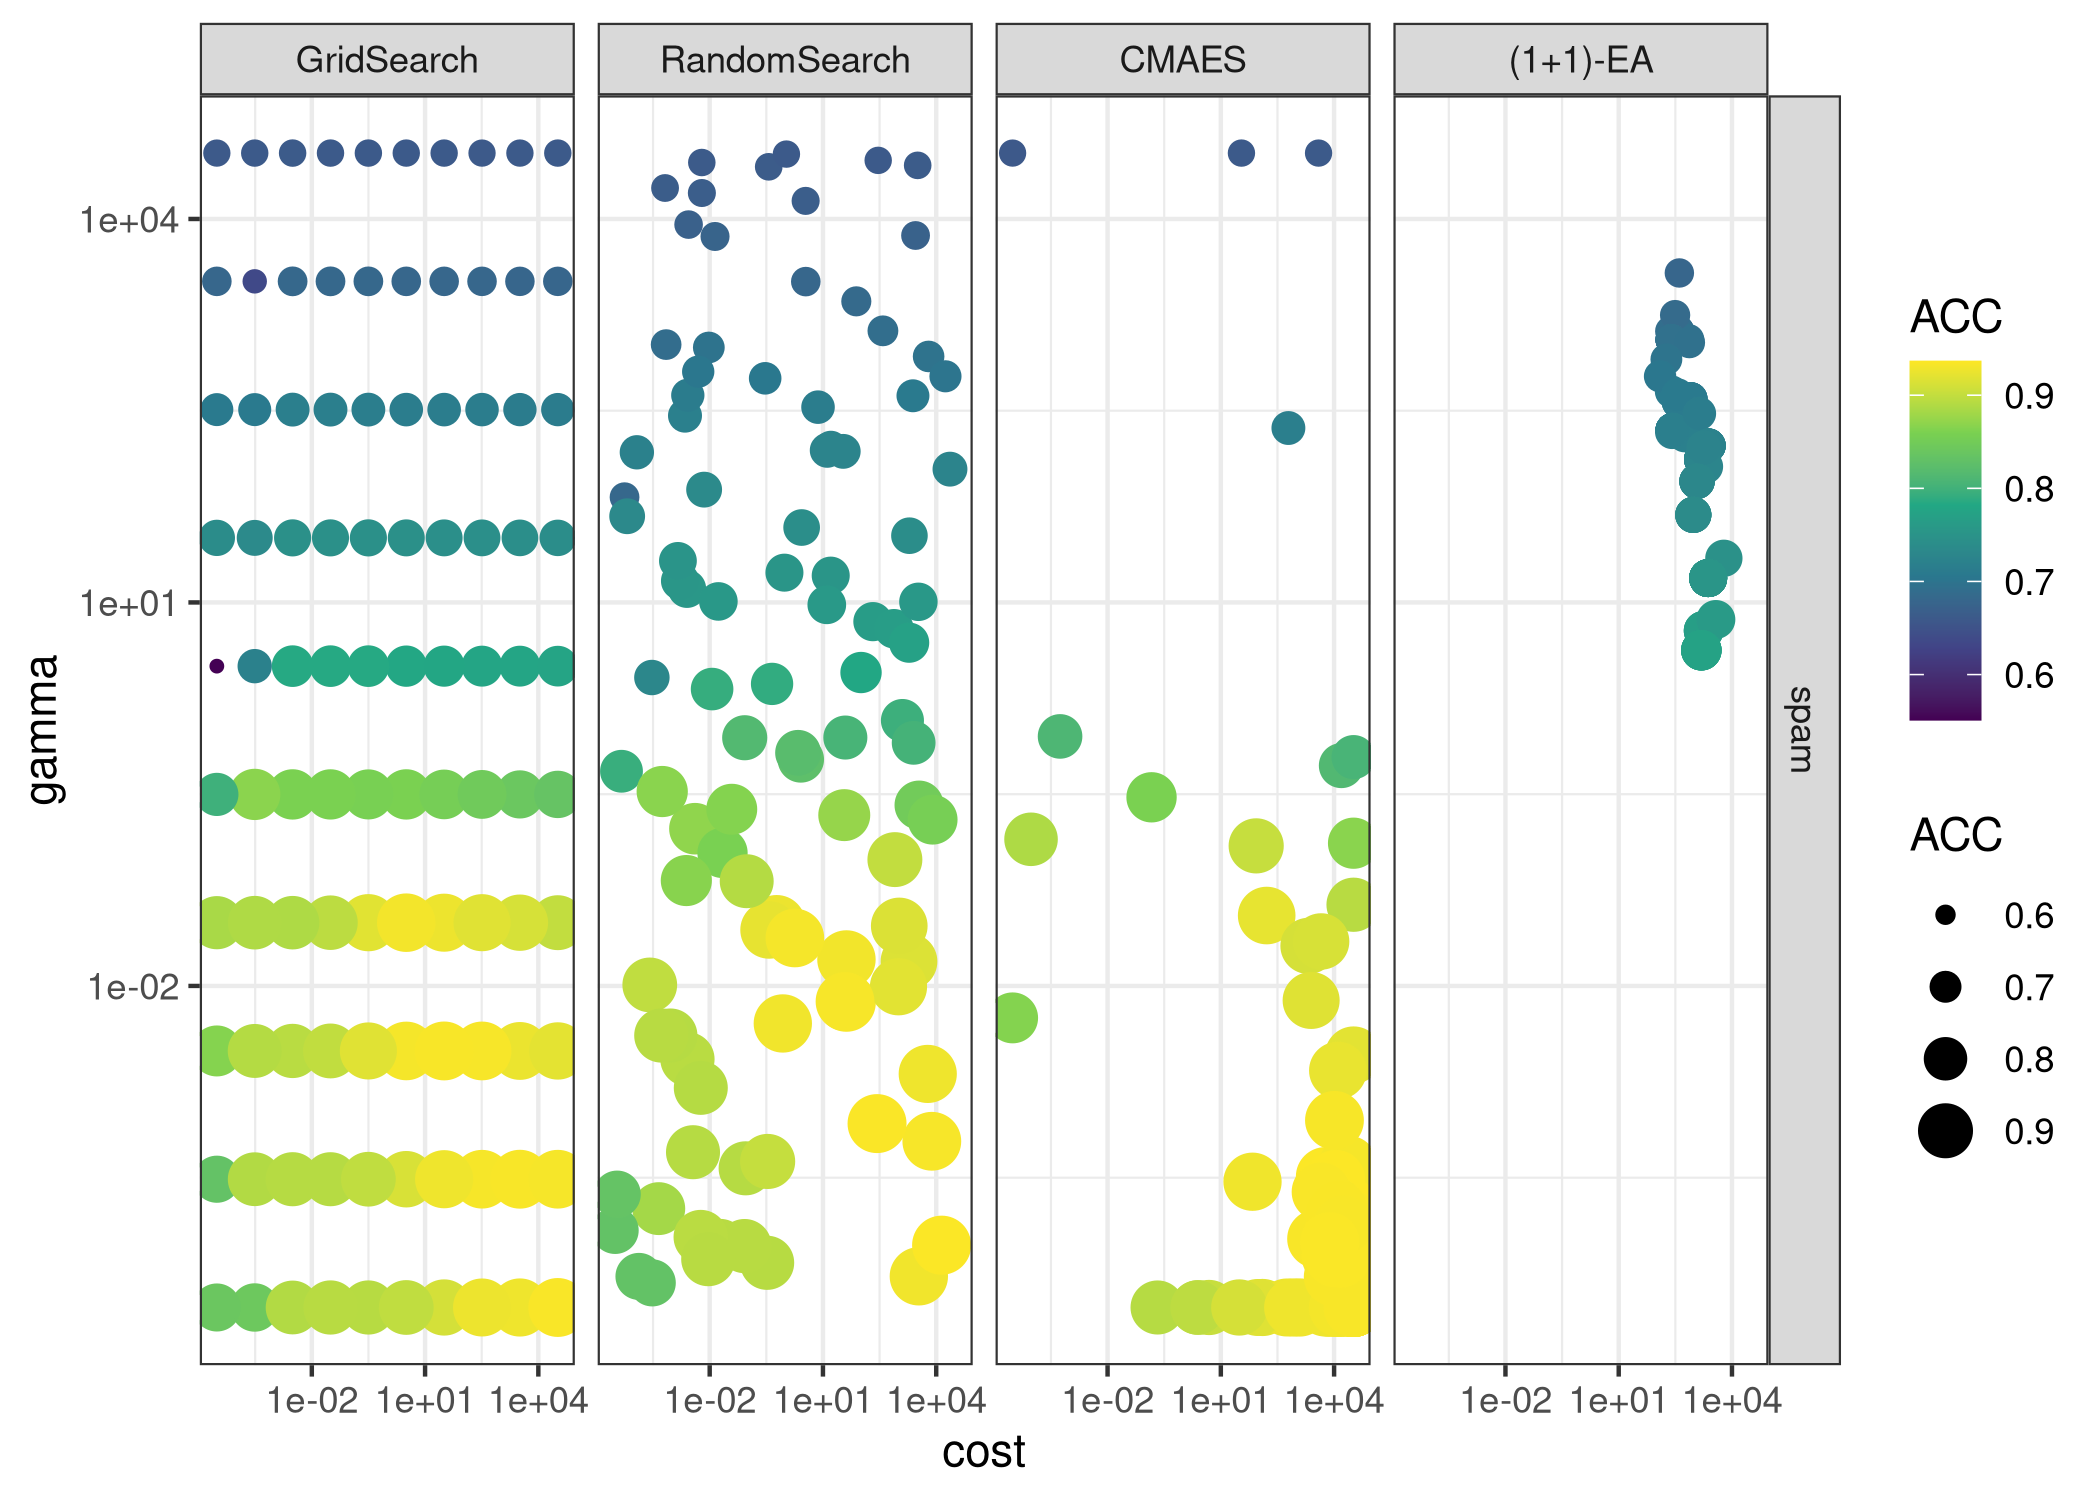
\includegraphics[width=0.9\textwidth]{figure/benchmark_scatter.png}
  \end{figure}
\end{column}
\end{columns}

\end{frame}
\begin{frame}{Tuning Example cont.}

The \emph{optimization trace} shows the best obtained performance until a given time point.
\begin{columns}
\begin{column}{0.4\textwidth}
  % \footnotesize
  \only<1>{

    % Note:

    \begin{itemize}
      \item For \emph{random search} and \emph{grid search} the chronological order of point evaluation is somewhat arbitrary
      \item The curve shows the performance on the tuning validation (\emph{inner resampling}) on a single fold
    \end{itemize}
  }
  \only<2>{
    \begin{itemize}
      \item The outer 10-fold CV gives us 10 optimization curves.
      \item The median at each time point gives us an estimate of the average optimization progress.
    \end{itemize}
  }
  % \only<4>{
    % \begin{itemize}
      % \item Remember: The final model will be trained on the \emph{outer training set} with the configuration $\finconf$ that lead to the best performance on the \emph{inner test set}.
      % \item To compare the effectiveness of the tuning strategies we have to look at the performance that $\finconf$ gives us on the \emph{outer test set}.
    % \end{itemize}
  % }
\end{column}
\begin{column}{0.6\textwidth}
  \vspace{-1em}
  \begin{figure}
  \only<1>{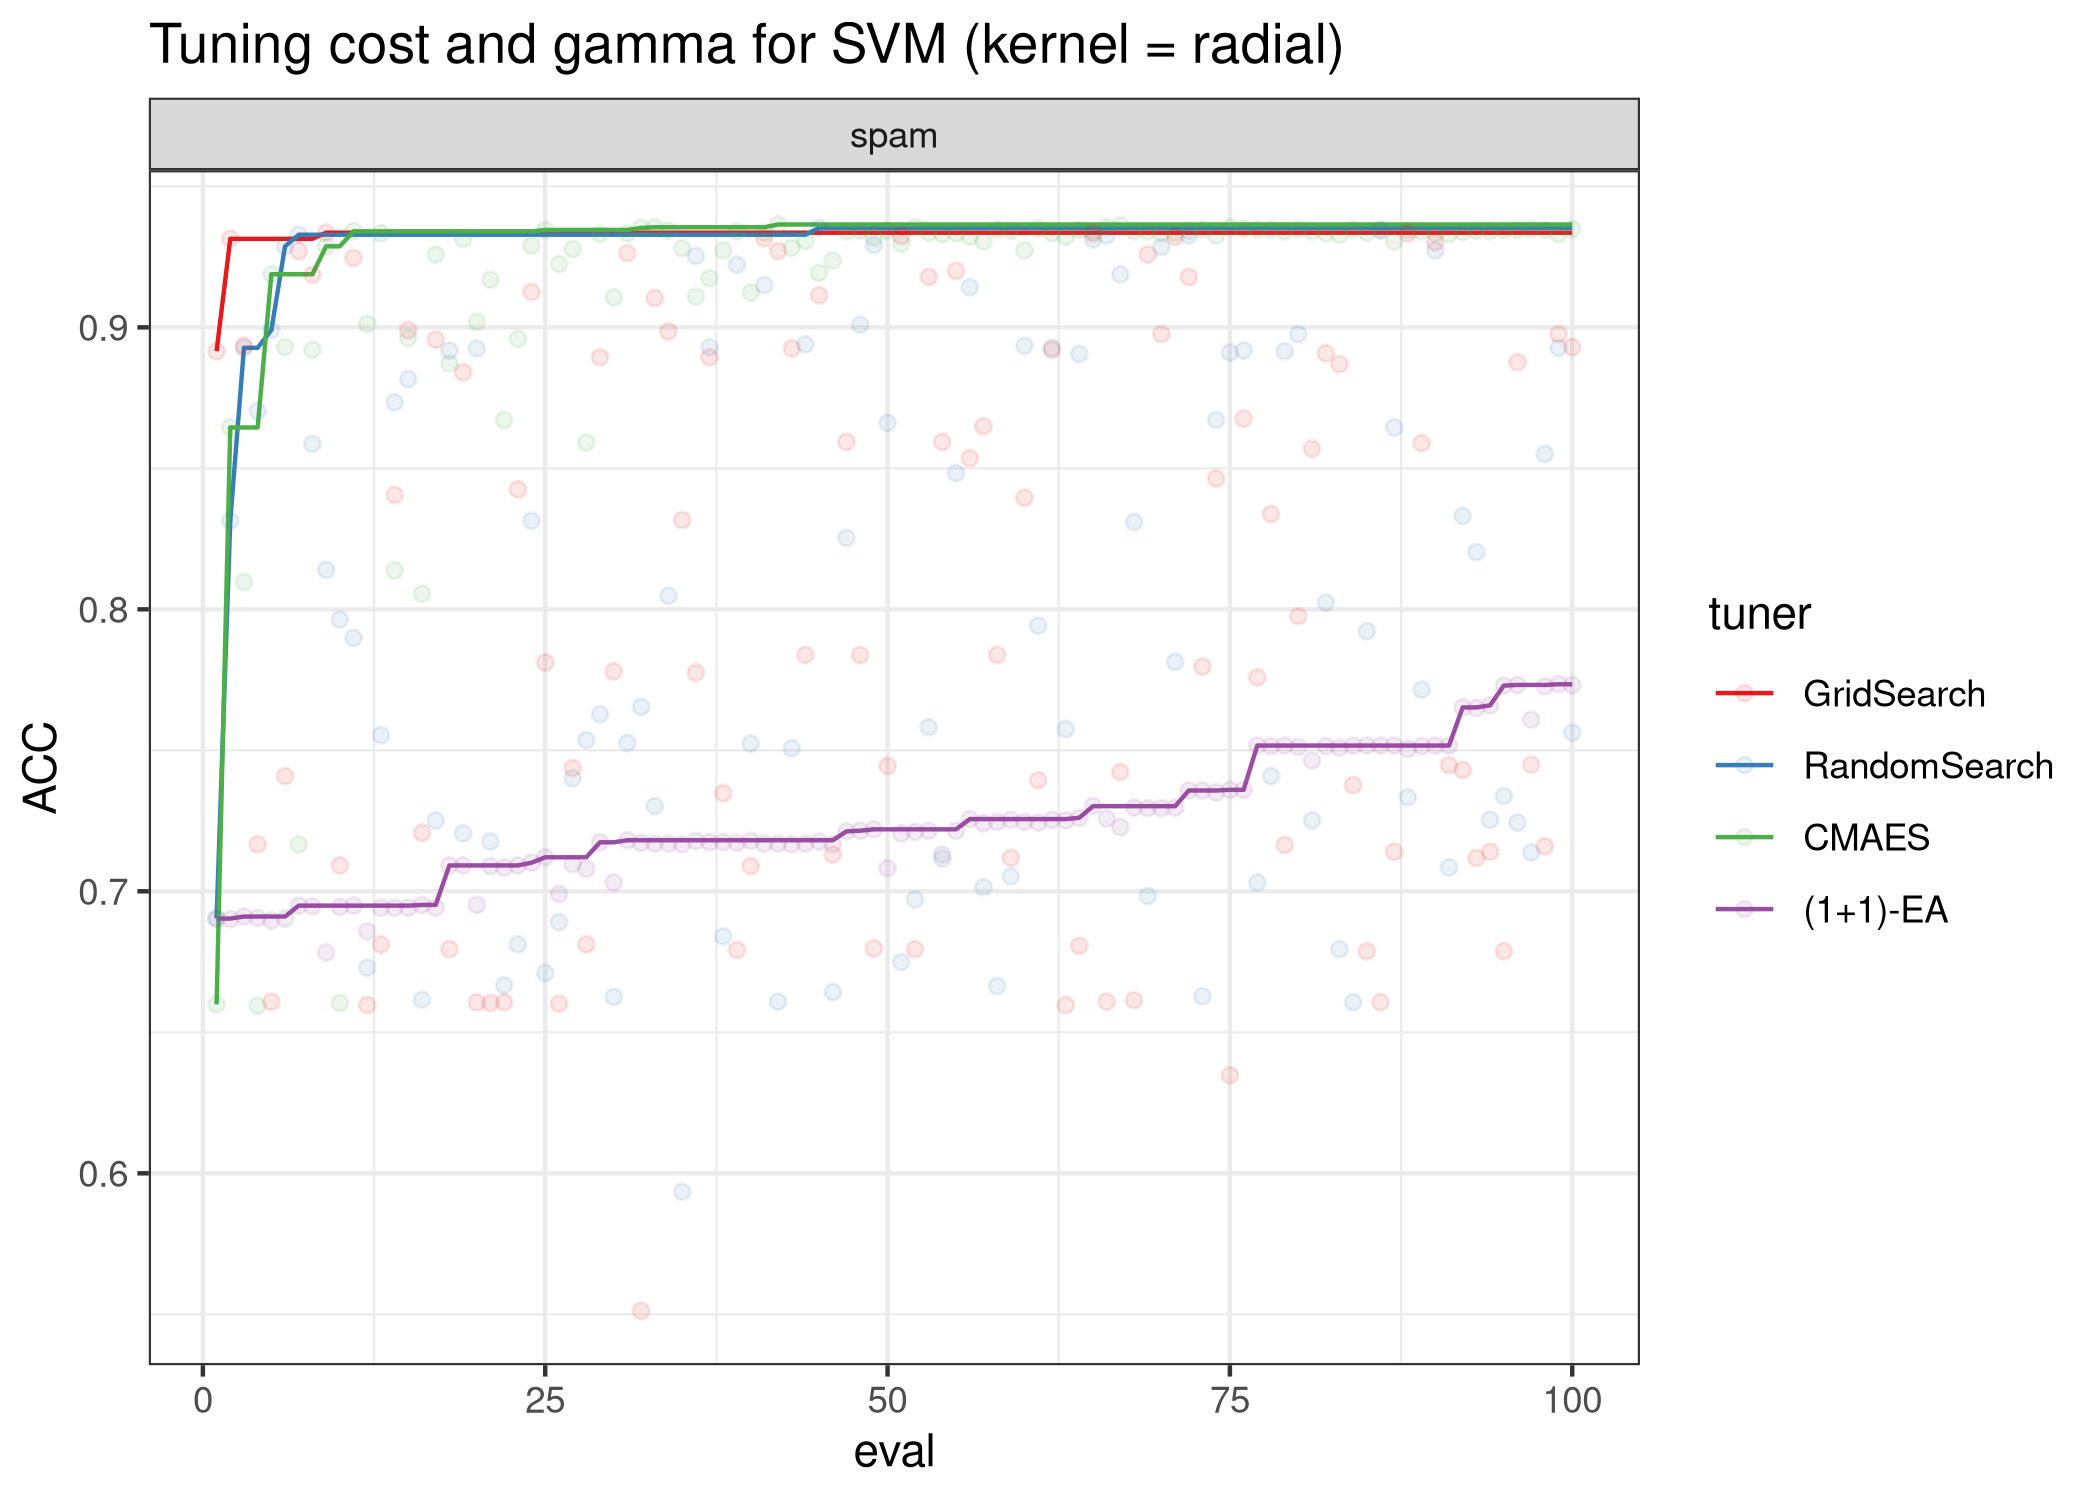
\includegraphics[width=\textwidth]{figure/benchmark_curve_iter_1.png}}
  % \only<2>{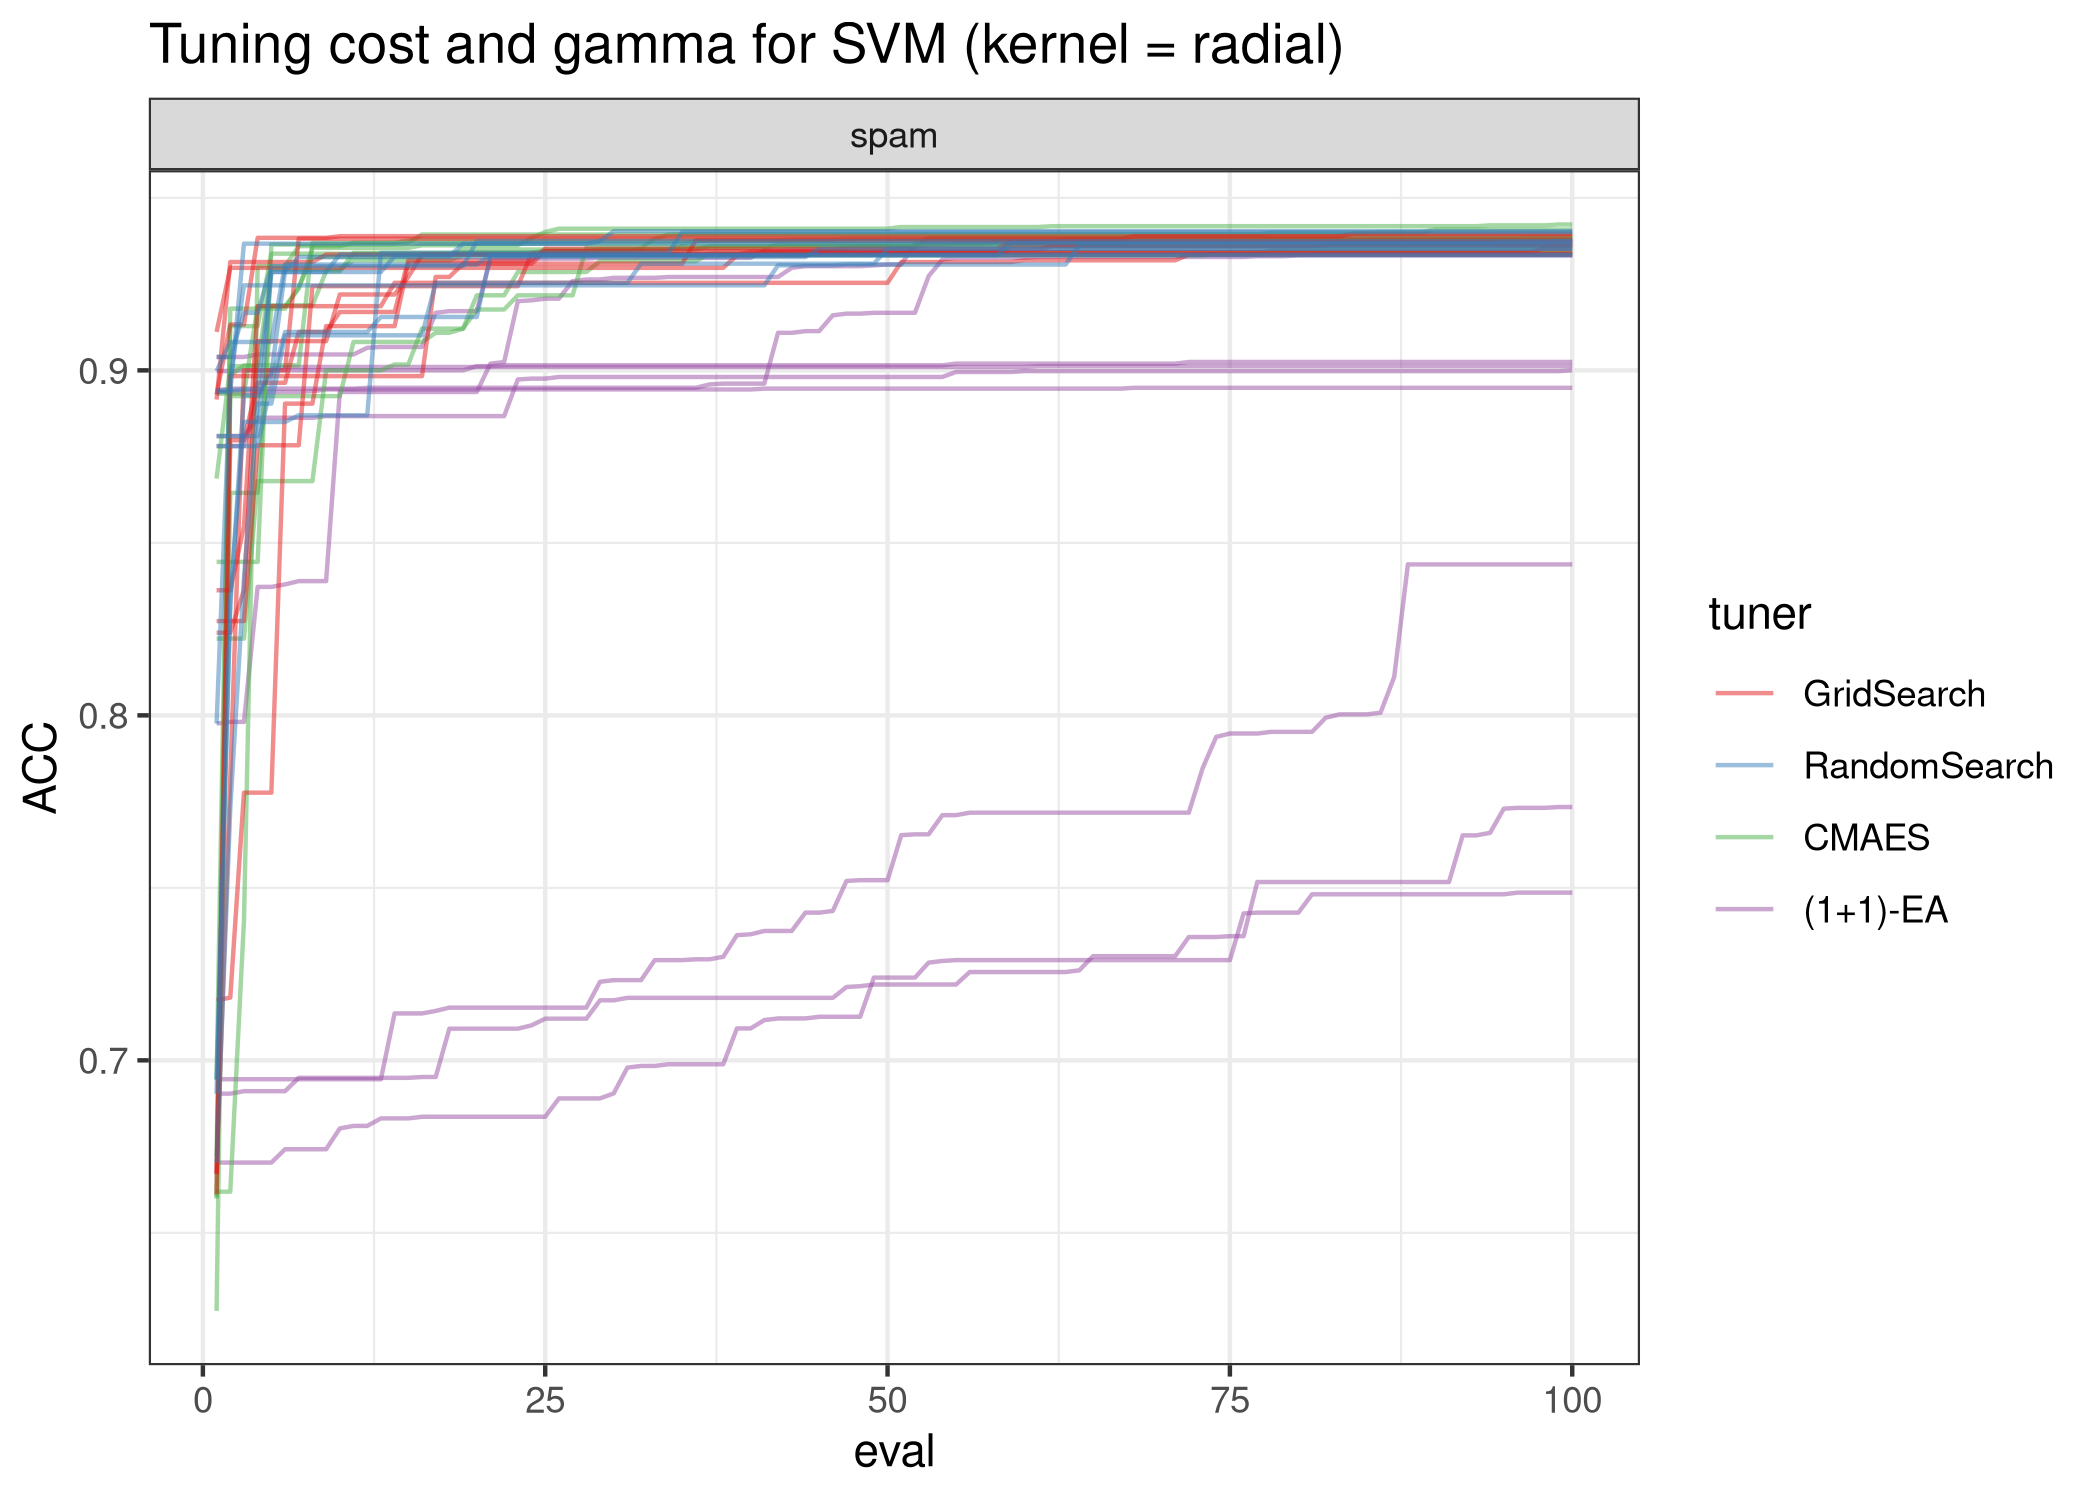
\includegraphics[width=\textwidth]{images/benchmark_curve_iter_all.png}}
  % \only<3>{\includegraphics[width=\textwidth]{images/benchmark_curve_median.png}}
  \only<2>{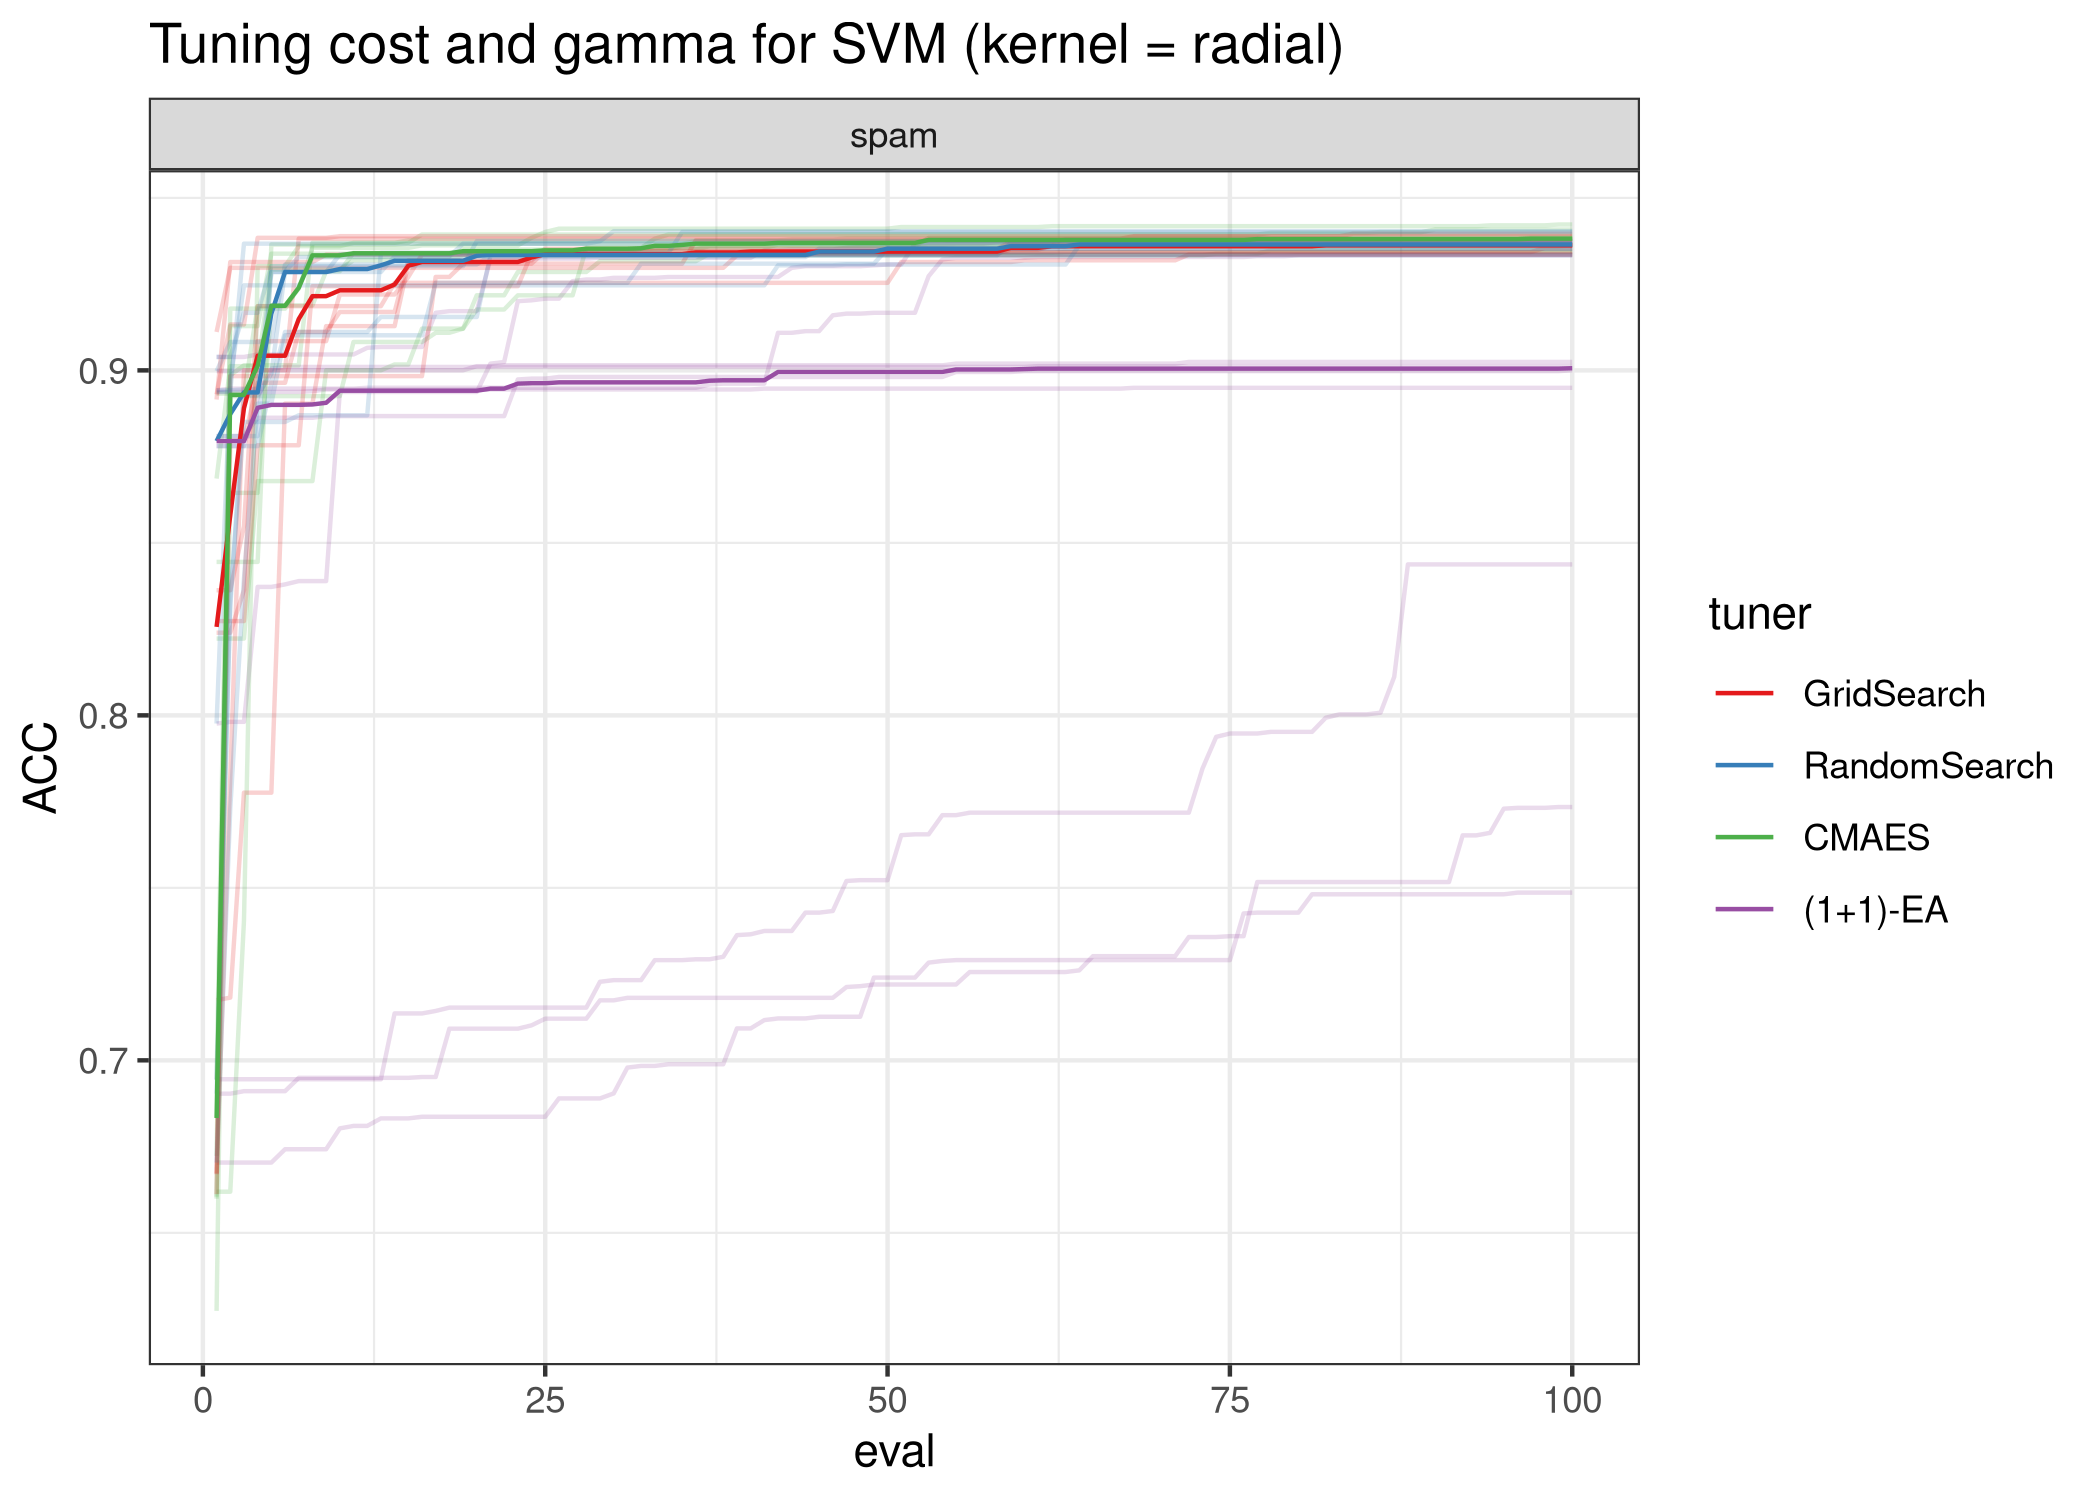
\includegraphics[width=\textwidth]{figure/benchmark_curve_iter_all_median.png}}
  \end{figure}
\end{column}
\end{columns}


  %   \footnotesize
  %     \item Tuning does not necessarily improve the performance of the learner, because e.g.\ tuning is badly configured or default values are determined by \emph{clever} heuristics.
  %     \item Tuning error can be overly optimistic (see \emph{nested resampling}).
  %   \end{itemize}
  % }
  % \only<2>{
  %   \begin{itemize}
  %     \item Effect of the chosen resampling split (objective noise) can dominate tuning effect.
  %   \end{itemize}
  % }
\end{frame}

\begin{frame}{Tuning Example: Validation}

\begin{columns}
\begin{column}{0.49\textwidth}
  % \footnotesize

  Distribution of the ACC-values on \emph{outer test sets} with a 10-fold CV.

  % Note:

  \begin{itemize}
      \item We compare with SVM in (unreasonable) defaults $(\text{cost}=1,\gamma=1)$ and the previously discussed heuristic with $\text{cost} = 1$
    \item We abstained from proper statistical testing here
    \item The performance is somewhat lower than indicated by the results on the inner resampling
  \end{itemize}

\end{column}
\begin{column}{0.49\textwidth}
  \vspace{-1em}
  \begin{figure}
  % \includegraphics[width=\textwidth]{images/benchmark_boxplot_tuners.png}
  % \includegraphics[width=\textwidth]{images/benchmark_boxplot_default.png}
  \includegraphics[width=\textwidth]{figure/benchmark_boxplot_all.png}
  \end{figure}
\end{column}
\end{columns}
\end{frame}

% \begin{frame}{Tuning Example: Validation}

% \begin{columns}
% \begin{column}{0.4\textwidth}
%   \footnotesize

%   % \begin{itemize}
%   % \end{itemize}
% \end{column}
% \begin{column}{0.6\textwidth}
%   \begin{figure}
%   \includegraphics[width=\textwidth]{images/benchmark_boxplot_default.png}
%   \end{figure}
% \end{column}
% \end{columns}
% \end{frame}


% \begin{frame}{Tuning Example: Validation}

% \begin{columns}
% \begin{column}{0.4\textwidth}
%   % \footnotesize

%   \begin{itemize}
%   \end{itemize}
% \end{column}
% \begin{column}{0.6\textwidth}
%   \begin{figure}
%   \includegraphics[width=\textwidth]{images/benchmark_boxplot_all.png}
%   \end{figure}
% \end{column}
% \end{columns}
% \end{frame}
%\begin{frame}{Practical Hints: Nested Resampling}
%\begin{itemize}
%   \item For small data sets the relative size of the \emph{inner training set} should not differ much from \emph{outer training set}. Example: \\$n = 200$,
%   \begin{itemize}
%     \item outer resampling: 5-fold CV, inner resampling: 3-fold CV: $n_{\text{inner train}} = \frac{4}{5} \cdot {2}{3} \cdot n = 0.53 * n = 107$
%     \item inner and outer resampling: 10-fold CV: $\frac{9}{10} \cdot \frac{9}{10} \cdot n = 0.81 * n = 162$
%   \end{itemize}
%   \item Resampling strategies depend on dataset sizes:
%  \begin{itemize}
%    \item Small datasets: More resampling iterations necessary to obtain reliable performance estimate (e.g.\ repeated CV).
%    \item Large datasets: Less resampling iterations possible due to runtime, but holdout can be sufficient to estimate performance.
%    \item For unbalanced and multi-class datasets $n$ has to be higher to obtain reliable performance estimates, i.e.\ they should be treated like small datasets if not sufficiently big.
%  \end{itemize}
%\end{itemize}
%\end{frame}

\begin{frame}[allowframebreaks]{Challenges and Final Comments}
\begin{enumerate}
  \item Getting it right which hyperparameters to tune, in what ranges, and where defaults and where heuristics might be ok.
  \item Choosing and balancing out budget for tuning and inner and outer resampling.
  \item Dealing with multi criteria-situations, where multiple performance metrics are of interest
  \item Dealing with parallelization and time-heterogeneity    
  \item Ensuring the computational stability of the tuning process and dealing with crashes
    
  %\framebreak    

  \item Post-Hoc analysis of all obtained tuning results
  \item Exploiting the multi-fidelity property of ML training (suppress bad configurations early without investing too much time)
  \item Including preprocessing and full pipelining into the tuning process, and dealing with complex hierarchical spaces
 \end{enumerate}

\end{frame}


\endlecture
\end{document}
